\documentclass{llncs}

\usepackage{todonotes}

\usepackage[utf8]{inputenc} \usepackage[T1]{fontenc}    \usepackage[
    colorlinks,
    linkcolor={red!50!black},
    citecolor={blue!50!black},
    urlcolor={blue!80!black}]{hyperref}       \usepackage{url}            \usepackage{booktabs}       \usepackage{amsfonts}       \usepackage{nicefrac}       \usepackage{microtype}      \usepackage{xcolor}
\usepackage{cleveref}
\usepackage{url}
\usepackage{inconsolata}
\usepackage{xspace}
\usepackage{wrapfig}
\usepackage{microtype}


\usepackage{graphicx}
\usepackage{tikz}
\usetikzlibrary{fit}

\newcommand{\rocq}{Rocq\xspace}
\newcommand{\petanque}{Pétanque\xspace}
\newcommand{\fleche}{Flèche\xspace}
\newcommand{\pytanque}{\texttt{pytanque}\xspace}

\newcommand{\coq}[1]{\mintinline{coq}{#1}}
\newcommand{\python}[1]{\mintinline{python}{#1}}

\newcommand{\gpto}{GPT-4o mini\xspace}
\newcommand{\claude}{Claude 3.5 Sonnet\xspace}
\newcommand{\oonemini}{o1 mini\xspace}
\newcommand{\oone}{o1\xspace}

\title{MiniF2F in Rocq: Automatic Translation Between Proof Assistants
    — A Case Study}

\author{Jules Viennot,\inst{1}
  Guillaume Baudart,\inst{1}\\
  Emilio Jesús Gallego Arias,\inst{1}
  Marc Lelarge\inst{2}
}

\institute{
IRIF, Université Paris Cité, Inria, CNRS \and
DI ENS, PSL University, Inria
}

\begin{document}

\maketitle

Recent LLMs have demonstrated impressive ability in proving theorems using interactive theorem provers~(ITP) such as Isabelle~\cite{DBLP:conf/nips/WuJLRSJS22,DBLP:journals/corr/abs-2303-04910}, Lean~\cite{DBLP:conf/iclr/PoluHZBBS23,DBLP:journals/corr/abs-2306-15626}, or Rocq~\cite{DBLP:journals/corr/abs-2305-04369,DBLP:journals/corr/abs-2412-14063}.
Unfortunately, fundamental differences between proof systems have resulted in diverse datasets, which makes the comparison between techniques developed for different proof assistant particularly challenging.

However, LLMs are particularly well fit for translating between programming languages that have extensive resources in common~\cite{DBLP:journals/corr/abs-2212-10079}.
In this work, we explore whether state-of-the-art LLMs can be leveraged to automatically translate a dataset of formal theorems from one proof assistant to another.
We focus on MiniF2F~\cite{zheng2021minif2f,2210.12283}, a dataset of  high-school-level problems that has already been formalized in Lean, Isabelle/HOL, and MetaMath.
This dataset is a popular benchmark for evaluating ML-based automated proof techniques~\cite{polu2020generative,thakur2024context,mikula2023magnushammer,wang2024proving}.
Despite previous attempts, this dataset has not yet been formalized in Rocq.\footnote{\url{https://github.com/openai/miniF2F/issues/66}}

In this work, we conduct an experiment using state-of-the-art LLMs to translate MiniF2F into Rocq. Our approach successfully translated 478 out of 488 theorems. The dataset is opensource: \url{https://github.com/LLM4Rocq/miniF2F-rocq}


\vspace{-0.5em}
\paragraph{Methodology}

The translation task focuses on generating a \rocq theorem
based on three sources:
a natural language description,
the Lean formalization, and
the Isabelle formalization.
Only theorem statements are considered,
proofs,
whether described in natural language or
formalized in Lean or Isabelle,
are deliberately ignored.
For each theorem we check that the result of the translation is a valid \rocq statement using Pétanque~\cite{nlir-mathai24}, a machine to machine interactive environment for \rocq.

We conducted our experiment in 3 stages of increasing complexity, from basic one-shot prompting to multi-turn conversations that incorporate feedback from unsuccessful attempts.
At each stage, we perform multiple rounds of translation using increasingly advanced models.
After each round, we verify that the generated codes matches the informal descriptions and the existing formalizations.
To limit the costs, the next round only focuses on theorems that remains untranslated.

\begin{itemize}
\item \emph{Stage 1: One-shot prompting.} We prompt the model with the natural language description of the theorem and the existing formalizations (Lean and Isabelle/HOL).
In this stage, we used \gpto, \claude, \oonemini, and \oone.
\item \emph{Stage 2: Multi-turn with errors.} The model can interact up to three times with the theorem provers.
Each new try incorporate the previous unsuccessful attempts and the error messages.
In this stage we used \claude and \oonemini.
\item \emph{Stage 3: Refined prompt.} We focus on \claude.
The prompt is refined to address common errors related to
complex numbers,
finite sums or products,
prime numbers,
the floor function,
and typing issues.
We increase the number of attempts to 6, and then 24.
\end{itemize}

\begin{figure}[t]
\centering
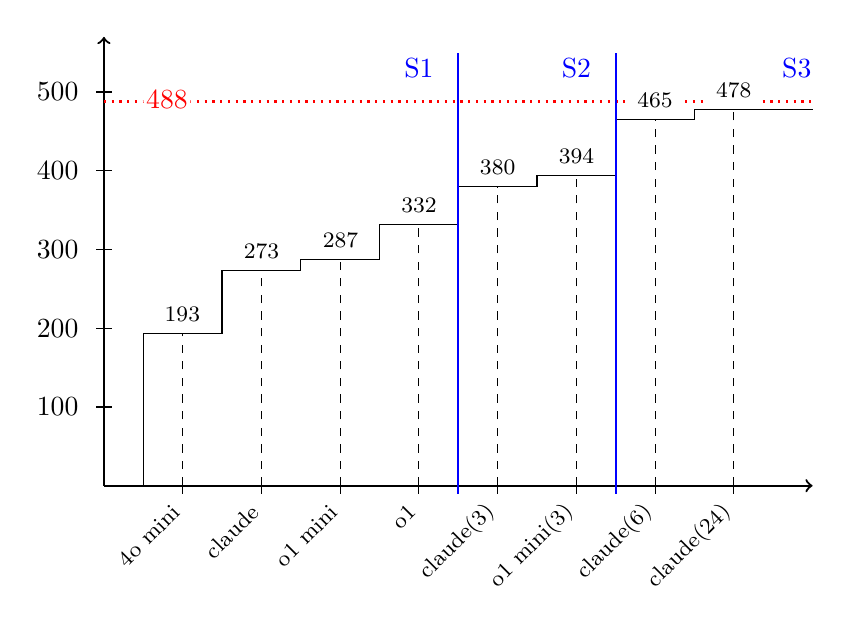
\begin{tikzpicture}

\draw[->, thick] (0,0) -- (9,0) node {};
    \draw[->, thick] (0,0) -- (0,5.7) node {};

\foreach \y in {100, 200, 300, 400, 500} {
        \draw (-0.1, \y/100) -- (0.1, \y/100);
        \node[left] at (-0.2, \y/100) {\y};
    }

\foreach \x/\label in {1/{4o mini}, 2/{claude}, 3/{\oonemini}, 4/{\oone}, 5/{claude(3)}, 6/{o1 mini(3)}, 7/{claude(6)}, 8/{claude(24)}} {
        \draw (\x, -0.1) -- (\x, 0.1);
        \node[rotate=45, left] at (\x, -0.2) {\footnotesize \label};
    }

\draw (0.5,    0) -- (0.5, 1.93)
       -- (1.5, 1.93) -- (1.5, 2.73)
       -- (2.5, 2.73) -- (2.5, 2.87)
       -- (3.5, 2.87) -- (3.5, 3.32)
       -- (4.5, 3.32) -- (4.5, 3.80)
       -- (5.5, 3.80) -- (5.5, 3.94)
       -- (6.5, 3.94) -- (6.5, 4.65)
       -- (7.5, 4.65) -- (7.5, 4.78)
       -- (9, 4.78);

    \draw[dotted, red, thick] (0, 4.88) -- (9, 4.88);
    \draw[text=red, thick, draw=none, fill=white] (0.8, 4.9) circle (3mm) node {488};

    \foreach \x/\y in {1/193, 2/273, 3/287, 4/332, 5/380, 6/394, 7/465, 8/478} {
      \node[fit={(\x - 0.35, \y / 100 + 0.01) (\x + 0.35, \y / 100 + 0.3)}, inner sep=0pt, draw=none, fill=white, thick] (rect) {\footnotesize \y};
      \draw[dashed] (\x, 0) -- (\x, \y / 100);
    }

\draw[blue, thick] (4.5, -0.1) -- (4.5, 5.5);
    \draw[blue, thick] (6.5, -0.1) -- (6.5, 5.5);

    \draw[text=blue, thick, draw=none, fill=white] (4, 5.3) circle (3mm) node {S1};
    \draw[text=blue, thick, draw=none, fill=white] (6, 5.3) circle (3mm) node {S2};
    \draw[text=blue, thick, draw=none, fill=white] (8.8, 5.3) circle (3mm) node {S3};

\end{tikzpicture}
 \caption{Translations of MiniF2F to Rocq, experimental results. For stages 2 and 3 we indicate the number of attempts in parenthesis.
}
\label{fig:results-minif2f}
\end{figure}

\vspace{-1em}
\paragraph{Results}
The cumulative results of each round are presented in \Cref{fig:results-minif2f}.
We observe that with basic one-shot prompting, we translate 68\% of the dataset requiring the use of the most advanced model \oone.
Stages 2 and 3 illustrate that the LLM can leverage successfully previous attempts.
At the end of our experiments only 10 theorems (2\% of the dataset) remains untranslated.

To validate our results, we asked an expert to compare the \rocq translations with the original Lean formalizations of a random sample of 50~theorems.
The expert found 6 discrepancies, but after inspection, the \rocq translation is also a correct formalization of the informal natural languages description of the problem.



\vspace{-0.5em}
\paragraph{Discussion}
We successfully used state-of-the-art LLMs to translate the MiniF2F dataset to \rocq.
However, while the translations are valid \rocq statements, it is possible that the resulting formalization makes the proof more challenging than in the other proof assistants.
We leave for future work a complete audit of all the theorems by experts \rocq users to mitigate this issue, but we believe that our work is a already a significant step forward.

\bibliographystyle{unsrt}
\bibliography{minif2f}

\newpage

\end{document}
